\documentclass[12pt]{article}

\setlength{\parindent}{0pt}
\setcounter{secnumdepth}{3}
\usepackage[margin=1in]{geometry}

% packages
\usepackage{amsmath, amsfonts, amsthm, amssymb}
\usepackage{graphicx, float}
\usepackage{mathtools}
\usepackage{titlesec}
\usepackage{interval}
\usepackage{hyperref}
\usepackage{siunitx}
\usepackage{titling}
\usepackage{vwcol}
\usepackage{setspace}
\usepackage{empheq}
\usepackage{cancel}
\usepackage{esdiff}
\usepackage{multicol}
\usepackage{mdframed}
\usepackage{esdiff}
\usepackage{tikzsymbols}
\usepackage{multicol}
\usepackage{tikz}
\usepackage{varwidth}
\usepackage{pgfplots}
\usepackage{fancyhdr}
\usepackage{enumitem}
\usepackage{tcolorbox}

\intervalconfig {
	soft open fences
}

% header
\pagestyle{fancy}
\fancyhf{}
\lhead{Ethan Fan}
\rhead{PCH}
\cfoot{\thepage}

% section format
\titleformat{\section}
  {\bfseries}
  {}
  {0em}
  {}
\titlespacing*{\section}{0pt}{0pt}{0.3em}

\titleformat{\subsection}[runin]
  {\bfseries}
  {}
  {0em}
  {}
\titlespacing*{\subsection}{0pt}{0pt}{0em}

\titleformat{\subsubsection}[runin]
  {\itshape}
  {(\roman{subsubsection})}
  {0em}
  {}

% commands
\newcommand{\alignedintertext}[1]{%
  \noalign{%
    \vskip\belowdisplayshortskip
    \vtop{\hsize=\linewidth#1\par
    \expandafter}%
    \expandafter\prevdepth\the\prevdepth
  }%
}

\newcommand*{\paren}[1]{\ensuremath\left(#1\right)}
\newcommand*{\limit}[2][x]{\ensuremath{\displaystyle\lim_{#1\to#2}}}
\newcommand*{\Limit}[3][x]{\ensuremath{\displaystyle\lim_{#1\to#2}\left[#3\right]}}
\newcommand*{\deriv}[1][x]{\ensuremath{\dfrac{\mathrm{d}}{\mathrm{d}#1}}}
\newcommand*{\Deriv}[2][x]{\ensuremath{\dfrac{\mathrm{d}}{\mathrm{d}#1}\left[#2\right]}}
\newcommand{\dydx}{\frac{dy}{dx}}
\newcommand*{\iinteg}[2][x]{\ensuremath{\displaystyle\int #2\;\mathrm{d}#1}}
\newcommand*{\dinteg}[4][x]{\ensuremath{\displaystyle\int_{#2}^{#3}#4\;\mathrm{d}#1}}
\newcommand*{\abs}[1]{\ensuremath{\left|#1\right|}}
\newcommand*{\eps}{\varepsilon}
\newcommand*{\real}{\ensuremath\mathbb{R}}
\newcommand*{\integer}{\ensuremath\mathbb{Z}}
\newcommand*{\posint}{\ensuremath\mathbb{Z^+}}
\newcommand*{\cbrt}[1]{\ensuremath{\sqrt[3]{#1}}}
\newcommand*{\lheqzero}{\ensuremath{\underset{\text{L'H}}{\overset{\left[\frac00\right]}{=}}}}
\newcommand*{\lheqinfty}{\ensuremath{\underset{\text{L'H}}{\overset{\left[\frac{\infty}{\infty}\right]}{=}}}}
\newcommand{\tor}{\text{ or }}
\newcommand{\floor}[1]{\lfloor #1 \rfloor}

\newcommand{\vem}{\vspace{0.5em}}
\newcommand{\example}[1]{\section{Example #1}}
\newcommand{\problem}[1]{\section{Problem #1}}
\newcommand{\subproblem}[1]{\subsection{(#1)} \,}

\DeclareMathOperator{\dne}{DNE}
\DeclareMathOperator{\sgn}{sgn}

\newcommand{\definition}[1]{\begin{tcolorbox}[colback=red!5!white,colframe=red!75!black,parbox=false] #1 \end{tcolorbox}}

\newcommand{\theorem}[2]{\begin{tcolorbox}[title={#1},colback=blue!5!white,colframe=blue!75!black,parbox=false] #2 \end{tcolorbox}}

\allowdisplaybreaks
% \postdisplaypenalty=100000

% document
\begin{document}

\vspace*{0cm}

% opening
\begin{center}
    {\Large \bfseries Problem Set 66} \\[0.5cm]
    {\large Significance of Derivative} \\[0.35cm]
    {\normalsize April 14, 2026}
\end{center}

% problems

\problem{6}
For each of the following functions, find the maximum and minimum values on the indicated intervals, by finding the critical points, and comparing the values at these points with the values at the endpoints. \vem

\subproblem{b} $f(x)=x^5+x+1$ on $[-1,1]$
\begin{gather*}
    f'(x)=5x^4+1 \implies f'(x)>0\\
    f(-1)=-1-1+1=-1\\
    f(1)=1+1+1=3\\
    \boxed{\max:(1,3),\min :(-1,-1)}
\end{gather*}

\subproblem{c} $f(x)=3x^4-6x^3+6x^2$ on $\left[ -\dfrac{1}{2}, \dfrac{1}{2} \right]$
\begin{gather*}
    f'(x)=12x^3-18x^2+12x\\
    6x(2x^2-3x+2)=0 \implies f'(0)=0\\
    f(0)=0\\
    f(-\frac{1}{2})=\frac{39}{16}\\
    f(\frac{1}{2})=\frac{15}{16}\\
    \boxed{\max:(-\frac{1}{2},\frac{39}{16}),\min :(\frac{1}{2},\frac{15}{16})}
\end{gather*}

\subproblem{d} $f(x)=\dfrac{1}{x^5+x+1}$ on $\left[ -\dfrac{1}{2}, 1 \right]$
\begin{gather*}
    f'(x)=-\frac{5x^4+1}{(x^5+x+1)^2} \implies f'(x)<0\\
    f(-\frac{1}{2})=\frac{32}{15}\\
    f(1)=\frac{1}{3}\\
    \boxed{\max:(-\frac{1}{2},\frac{32}{15}),\min :(1, \frac{1}{3})}
\end{gather*}

\subproblem{f} $f(x)=\dfrac{x}{x^2-1}$ on $[0,5]$
\begin{gather*}
    f'(x)= \frac{-x^2-1}{(x^2-1)^2} \implies f'(x)<0, \ x \ne 1\\
    f(1) \dne \\
    f(0)=0\\
    f(5)= \frac{5}{24}\\
    \boxed{\max: \dne ,\min : \dne}
\end{gather*}

\problem{7} \vspace{-0.5em}
(Calculator) Sketch the graph of the function $f(x)=x+\dfrac{3}{x^2}$ and find all local minimum and maximum points (This is the skill required for the AP Calculus exam).
\begin{gather*}
    f'(x)=0 \implies x=1.817\\
    \boxed{\text{local }\min :(1.817,2.726) }
\end{gather*}

\problem{10}
When a foreign object lodged in the trachea (windpipe) forces a person to cough, the diaphragm thrusts upward, causing an increase in pressure in the lungs. This is accompanied by a contraction of the trachea, making a narrower channel for the expelled air to flow through. For a given amount of air to escape in a fixed time, it must move faster through the narrower channel than the wider one. The greater the velocity of the airstream, the greater the force on the foreign object. X-rays show that the radius of the circular tracheal tube contracts to about two-thirds of its normal radius during a cough. According to a mathematical model of coughing, the velocity $v$ of the airstream is related to the radius $r$ of the trachea by the equation
\[
v(r) = k(r_0 - r)r^2, \quad \frac{r_0}{2} \le r \le r_0
\]
where $k$ is a constant and $r_0$ is the normal radius of the trachea. The restriction on $r$ is due to the fact that the tracheal wall stiffens under pressure and a contraction greater than $\dfrac{r_0}{2}$ is prevented (otherwise the person would suffocate). \vem

\subproblem{a} Determine the value of $r$ in the interval $\left[ \dfrac{r_0}{2}, r_0\right]$ at which $v$ has an absolute maximum. How does this compare with experimental evidence?
\begin{gather*}
    v(r)=k(-r^3+r_0r^2)\\
    v'(r)=k(-3r^2+2r_0r)=kr(2r_0-3r)\\
    \boxed{r=\frac{2r_0}{3}}
\end{gather*}
The value of $r$ falls within the range of restriction. Moreover, it perfectly aligns with the experimental value of about two-thirds of the normal radius. 

\subproblem{b} What is the absolute maximum value of $v$ on the interval?
\begin{align*}
    v(\frac{2r_0}{3})&=k(r_0-\frac{2r_0}{3})(\frac{2r_0}{3})^2\\
    &=k(\frac{r_0}{3})(\frac{4r_0^2}{9})\\
    &=\boxed{\frac{4kr_0^3}{27}}
\end{align*}

\subproblem{c} Sketch the graph of $v$ on the interval $[0, r_0]$.
\begin{figure}[H]
    \centering
    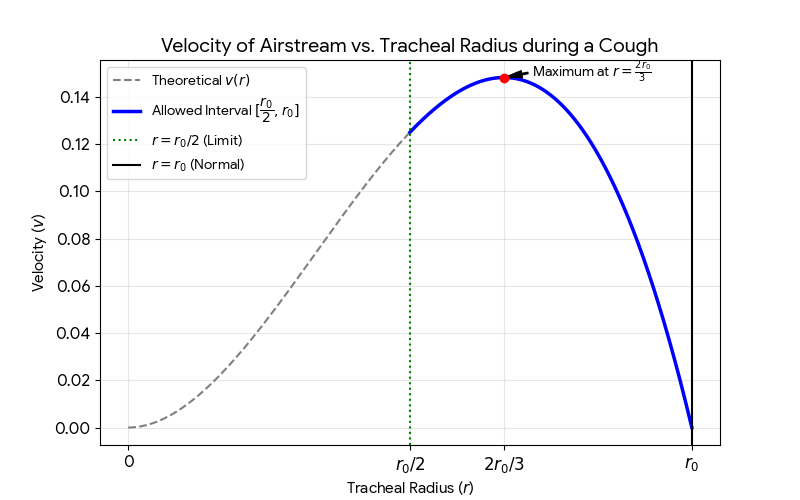
\includegraphics[width=0.6\linewidth]{vgraph.png}
\end{figure}

\problem{11}
(Optional) Rainbows are created when raindrops scatter sunlight. They have fascinated mankind since ancient times and have inspired attempts at scientific explanation since the time of Aristotle. In this project we use the ideas of Descartes and Newton to explain the shape, location, and colors of rainbows. \vem

PART 1: \vem

The figure 5 shows a ray of sunlight entering a spherical raindrop at A. Some of the light is reflected, but the line $AB$ shows the path of the part that enters the drop. Notice that the light is refracted toward the normal line $AO$ and in fact Snell's Law says that $\sin\alpha = k\sin\beta$, where $\alpha$ is the angle of incidence, $\beta$ is the angle of refraction, and $k \approx 4/3$ is the index of refraction for water. At $B$ some of the light passes through the drop and is refracted into the air, but the line $BC$ shows the part that is reflected. (The angle of incidence equals the angle of reflection.) When the ray reaches $C$, part of it is reflected, but for the time being we are more interested in the part that leaves the raindrop at $C$. (Notice that it is refracted away from the normal line.) The angle of deviation $D(\alpha)$ is the amount of clockwise rotation that the ray has undergone during this three-stage process. Thus
\[
D(\alpha) = (\alpha - \beta) + (\pi - 2\beta) + (\alpha - \beta) = \pi + 1\alpha - 4\beta
\]
Show that the minimum value of the deviation $D(\alpha) \approx 138^\circ$ is and occurs when $\alpha \approx 59.4^\circ$. The significance of the minimum deviation is that when $\alpha \approx 59.4^\circ$ we have $D'(\alpha) \approx 0$, so $\Delta D/\Delta \alpha$. This means that many rays with $\alpha \approx 59.4^\circ$ become deviated by approximately the same amount. It is the concentration of rays coming from near the direction of minimum deviation that creates the brightness of the primary rainbow. The figure above shows that the angle of elevation from the observer up to the highest point on the rainbow is $180^\circ - 138^\circ = 42^\circ$. (This angle is called the rainbow angle.)
\begin{gather*}
    D(\alpha)=\pi + 2\alpha - 4\beta=\pi+2\alpha - 4\arcsin \paren{\frac{3\sin \alpha}{4}}\\
    D'(\alpha )=2- \frac{4}{\sqrt{1-(\frac{3\sin \alpha}{4})^2}} \cdot \frac{3}{4}\cos \alpha =2-\frac{12\cos \alpha}{\sqrt{16-9\sin ^2 \alpha }}\\
    D'(\alpha)=0 \implies \frac{12\cos \alpha}{\sqrt{16-9\sin ^2 \alpha }}=2\\
    6\cos \alpha = \sqrt{16-9\sin ^2 \alpha }\\
    36\cos^2 \alpha = 16-9\sin ^2 \alpha\\
    \cos^2 \alpha = \frac{7}{27}\\
    \boxed{\alpha = \arccos \sqrt{\frac{7}{27}}}
\end{gather*}

\end{document}

